\documentclass[10pt,a4paper]{article}
\usepackage[utf8]{inputenc}
\usepackage[T1]{fontenc}
\usepackage{lmodern}
\usepackage[margin=1.5cm, top=1.4cm, bottom=1.4cm]{geometry}
\usepackage{hyperref}
\usepackage{enumitem}
\usepackage{titlesec}
\usepackage{xcolor}
\usepackage{graphicx}

\definecolor{accent}{HTML}{00686E}
\hypersetup{colorlinks=true, urlcolor=accent, linkcolor=accent}
\pagenumbering{arabic}
\setlength{\parindent}{0pt}

\titleformat{\section}{\large\bfseries\color{accent}}{}{0em}{}[\vspace{-0.6em}\rule{\textwidth}{0.8pt}]
\titlespacing{\section}{0pt}{7pt}{4pt}

\newcommand{\role}[4]{%
  \textbf{#1} \hfill \textbf{#2}\\[1pt]%
  \textit{#3} \hfill \textit{#4}\\[2pt]%
}
\setlist[itemize]{leftmargin=1.2em, itemsep=1.5pt, topsep=2pt, parsep=0pt}

\begin{document}

% ================= HEADER =================
\begin{minipage}[c]{0.80\textwidth}
  {\Huge\bfseries Prabhavit Gupta}\\[3pt]
  {\color{accent}\large AI-First QA Engineer: Playwright Automation, TypeScript \& Agentic Systems}\\[6pt]
  {\footnotesize +39 351 610 7807 ~$\vert$~
  \href{mailto:prabhavitg@gmail.com}{prabhavitg@gmail.com} ~$\vert$~
  \href{https://www.linkedin.com/in/prabhavit/}{linkedin.com/in/prabhavit} ~$\vert$~
  \href{https://github.com/prab-gupta}{github.com/prab-gupta} ~$\vert$~
  Venice, Italy (EU Permanent Resident / Global Remote Ready)}
\end{minipage}\hfill
\begin{minipage}[c]{0.18\textwidth}
  \raggedleft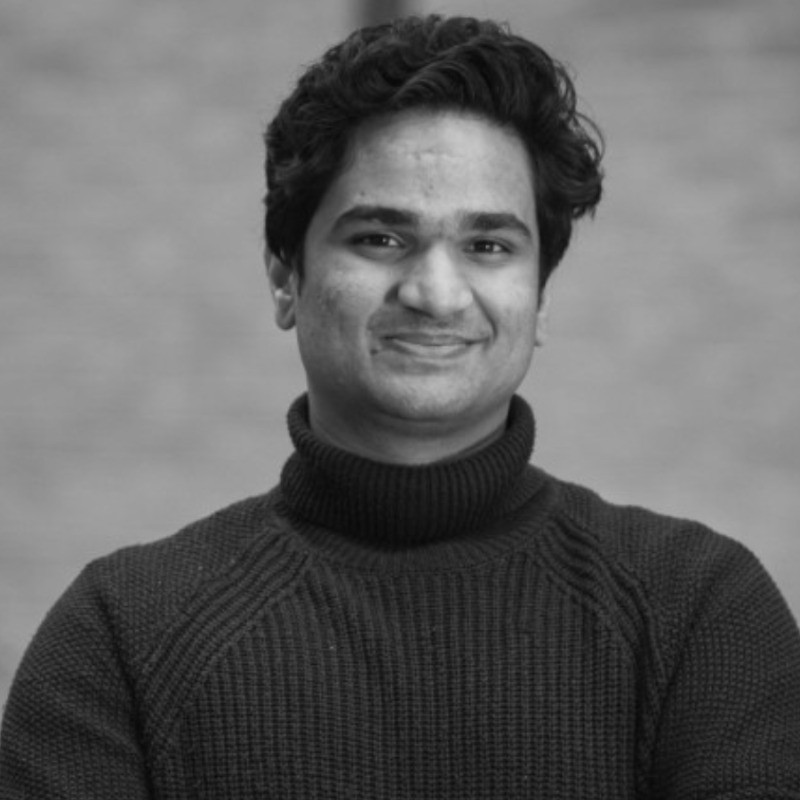
\includegraphics[width=2.0cm]{photo.jpg}
\end{minipage}
\vspace{-2pt}

% ================= SUMMARY =================
\section{Summary}
QA Automation and AI Systems Engineer with 3 years of hands-on production experience architecting end-to-end test automation frameworks, regression test suites, and AI evaluation pipelines. Deep expertise in Playwright (TypeScript/Python), API contract verification, and automated regression testing for customer-facing AI agents and distributed web applications. Proven track record embedding AI-driven testing workflows to accelerate test design, automate scenario coverage, and validate non-deterministic LLM behavior against ground-truth benchmarks. Holder of an EU Long-Term Residence Permit (permanent unrestricted EU work authorization across all EU member states, no sponsorship required); based in Venice, Italy and available immediately for remote roles.

% ================= TECHNICAL EXPERTISE =================
\section{Technical Expertise}
\begin{itemize}
  \item \textbf{Test Automation Frameworks:} Playwright (TypeScript \& Python), End-to-End (E2E) testing, API contract testing, component testing, regression test suite maintenance, headless CI browser automation.
  \item \textbf{AI-First Quality Assurance \& Evaluation:} LLM evaluation harnesses, transcript verification, ground-truth benchmark datasets, hallucination and grounding detection, AI coding tools (Claude Code, GitHub Copilot).
  \item \textbf{Software Development \& Programming:} TypeScript, Python, Node.js, RESTful API testing (Playwright API, Postman), JSON schema validation, asynchronous execution patterns.
  \item \textbf{DevOps \& Version Control:} Git branching workflows, GitHub Actions / CI/CD pipelines, Docker containerization, test reporting, error logging and root-cause analysis.
  \item \textbf{Languages \& Work Authorization:} English (C1 Professional, fluent), Hindi (Native), Italian (Beginner). EU Long-Term Residence Permit (unrestricted EU work authorization across all EU member states, no sponsorship required).
\end{itemize}

% ================= EXPERIENCE =================
\section{Experience}

\role{\href{https://flowspace.co}{FlowSpace.co}}{Mar 2024 - Aug 2026}{Lead Developer \& AI Systems Architect}{London, UK (remote)}
\begin{itemize}
  \item Architected and maintained comprehensive automated test suites using Playwright and TypeScript for a platform serving 4,500+ active enterprise users, covering UI flows, authentication, and REST APIs.
  \item Built specialized automated evaluation harnesses to test customer-facing AI agents and RAG pipelines against ground-truth datasets, systematically catching regressions in reasoning and tool-calling schemas.
  \item Integrated automated Playwright test execution into CI/CD pipelines, achieving high test reliability, flake reduction, and zero functional regressions across continuous deployment releases.
  \item Implemented schema validation pipelines for document parsing and data ingestion, ensuring inbound partner payloads adhered strictly to expected data contracts.
  \item Partnered closely with engineering and product teams to define test plans, triage production incident reports, and implement preventive regression checks.
\end{itemize}

\role{Urlink}{Apr 2025 - Jul 2025}{Project Manager \& Solutions Developer (Freelance)}{Barcelona, Spain (remote)}
\begin{itemize}
  \item Led technical discovery and implementation of customized web solutions and automated data processing pipelines for European client platforms.
  \item Established automated API validation suites and integration checks connecting third-party partner APIs to PostgreSQL databases, guaranteeing data consistency.
  \item Built functional prototypes and test environments to validate edge cases and user journeys prior to full sprint development.
\end{itemize}

\role{Independent Technical Consultant}{Aug 2023 - Feb 2024}{AI Automation \& Integration Developer}{Venice, Italy}
\begin{itemize}
  \item Developed and deployed custom automated integration test scripts, webhook listeners, and LLM extraction pipelines using TypeScript, Python, and n8n.
  \item Replaced brittle manual verification processes with automated regression test flows, featuring robust retry mechanisms, error alerting, and structured reporting.
  \item Documented testing procedures, test coverage matrices, and API contracts for client engineering teams.
\end{itemize}

% ================= EDUCATION =================
\section{Education}
\role{Ca' Foscari University of Venice}{2020 - 2024}{BA in Philosophy, International Studies and Economics}{Venice, Italy}
\begin{itemize}
  \item Rigorous training in formal logic, epistemology, analytical problem solving, and complex systems analysis.
\end{itemize}

\end{document}
